\documentclass[ oneside,% the name of the author
                    author={Cassie Qing Tang},
                % the degree programme: BSc, MEng, MSci or MSc.
                    degree={BSc},
                % the dissertation    title (which cannot be blank)
                     title={The Report for 3D Modelling of Queens Library \\ },
                % the dissertation subtitle (which can    be blank)
                    subtitle={ }]{dissertation}

\usepackage[english]{babel}
\usepackage[nottoc]{tocbibind}
\usepackage{graphicx}
\usepackage{subcaption}
\usepackage{float}
\usepackage[list=true]{subcaption}
\usepackage{caption}
\captionsetup[figure]{labelformat=empty} % This disables automatic labelling of graphics
\captionsetup[subfigure]{labelformat=empty} % This disables automatic labelling of graphics

\begin{document}

\maketitle
\fronmatter

\chapter*{Abstract}
This project targets the growing threat of online pet scams by creating an automated system to waste scammers' time and resources, aiding in scam identification and prevention. Following extensive development and testing, a four-week experimental deployment against pet scammers unveiled and refined effective scam-baiting tactics.

\chapter*{Acknowledgements}
I would like to express my special thanks to my supervisor, Dr Matthew Edwards, for his help and guidance in this project.
\\
\\
I would also like to give my thanks to School of Engineering for inviting me into UoB Computer Science OpenAI Team, which reimburses me the cost of using the different APIs of OpenAI.
\\
\\
Sign up for GitHub Student Developer Pack provides me free access to many useful tools, involving Maligun and Name.com. Appreciate the resources it provides!

\makedecl


\tableofcontents
\listoffigures
\listoftables

\chapter*{Ethics Statement}
An ethics application for this project was reviewed and approved by the faculty research ethics committee as application 17599.


\chapter*{Supporting Technologies}
I created my system based on an open-source GitHub repository from \url{https://github.com/an19352/scambaiter_back}. I extended and altered its code to fit my needs.
\\
\\
I integrated two GPT models, specifically GPT-3.5-turbo-0125 and GPT-4-0125-preview, into my system via their APIs to ensure the functionality of an automatic email reply feature. One necessary API key was acquired and configured using the resources available at \url{https://openai.com/}.
\\
\\
I applied my own domain name from \url{https://www.name.com/} in order to generate a large number of bait-email addresses.
\\
\\
I obtained a mailgun API key and build a mailbox server on \url{https://www.mailgun.com/}, which can support emails receiving, sending and tracking.

\chapter*{Notation and Acronyms}
\begin{quote}
\noindent
\begin{tabular}{lcl}
AFF                 &:     & Advance Fee Fraud    
 \\ 
HTTP/HTTPS          &:     & Hypertext Transfer Protocol/Hypertext Transfer Protocol Secure
 \\ 
HTML                &:     & Hypertext Markup Language
\\
XML                 &:     & Extensible Markup Language
\\
Regex               &:     & Regular Expression
\\
NLP                 &:     & Natural Language Processing
\\
SSL                 &:     & Secure Sockets Layer
\\
JSON                &:     & JavaScript Object Notation
\\
A*                  &:     & A-star
\\
GPT                 &:     & Generative Pre-Trained Transformer
\\
API/APIs            &:     & Application Programming Interface
\\
URL/url             &:     & Uniform Resource Locator


\end{tabular}
\end{quote}


\mainmatter

\chapter{Introduction}
\label{chap:context}


\chapter{Technical Background}
\section{Petscams.com}
The data for pet scam websites in this study was sourced from a volunteer organisation called \url{petscams.com}. This organisation operates a website, using the same domain name, to list fraudulent pet sales and shipping sites \cite{brady_fighting_2024}. \url{Petscams.com} is an effective and free platform offering a range of security services to alert the public about the danger of those websites. These services include victim reporting and comment systems, fraudulent website analysis, verification, classification, and continuous article updates. They also provide access of these data to law enforcement agencies to better disrupt and combat scammer activities. Beyond that, they have been a valuable resource for other researchers. For instance, their victim report system significantly contributed to a pet scam case study published in 2020 \cite{whittaker_understanding_2020}.
\\

Figure 1 illustrates how articles on this website maintain consistent HTML structural features in the developer mode of the Chrome browser. It's clear to see each article is nested within an $<$article$>$ tag, which is part of the HTML5 semantic markup, used to define independent content modules on the website. Importantly, each article's title, which the suspected fraudulent domain information, is placed within the $<$h2$>$ tag. 
\\

Furthermore, as shown in Figure 2 and Figure 3, the page layout across different articles is also remarkably uniform. Each article segments the key points and introductory content, ensuring information is presented clearly. The breakdown of each scam website in the article consists of four main parts - identity, review credibility, legality, and recommended next steps - for in-depth description and analysis. This thoughtful design considerably assists victims and researchers, in quickly and fully understanding the workings of pet scams.
\begin{figure}[!htb]
    \centering
    % First bigger subfig
    \begin{subfigure}[b]{0.7\textwidth}
        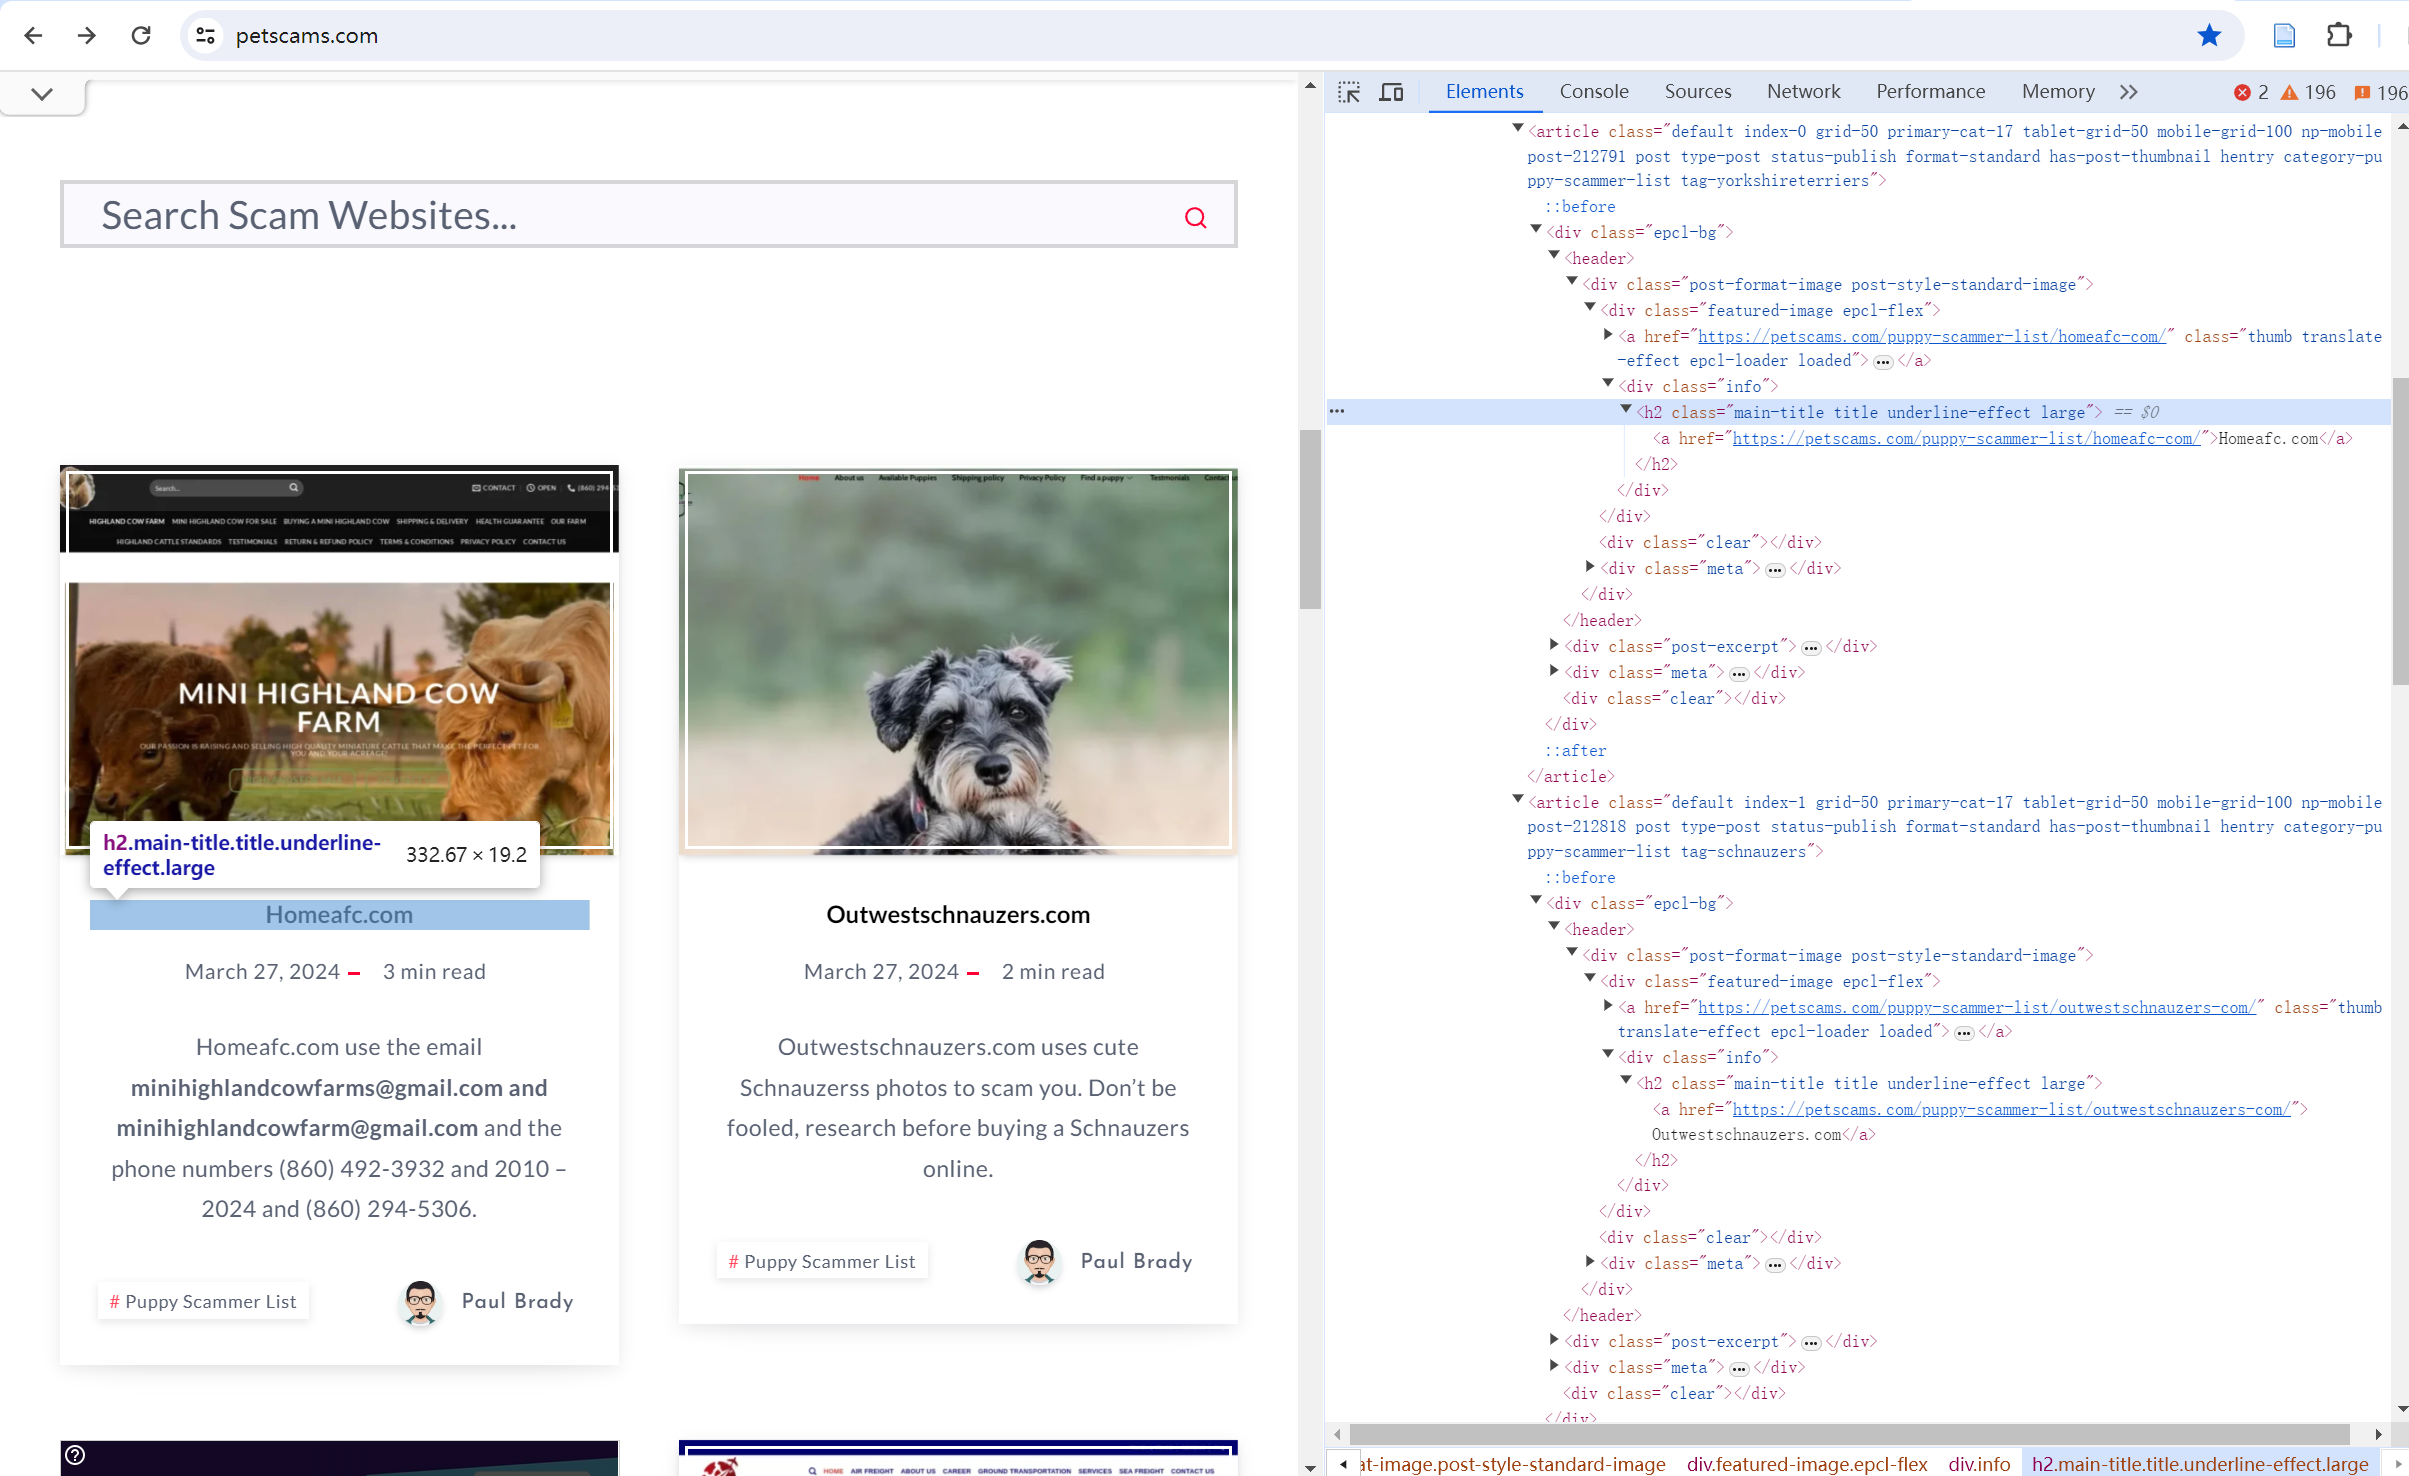
\includegraphics[width=\linewidth,height=0.28\textheight]{pic/figure1.png}
        \label{fig:petscams}
    \end{subfigure}
    \caption{Figure 1: Petscans.com in the developer mode}
    \label{fig:main1}
\end{figure}

\begin{figure}[!htb]\ContinuedFloat
    \centering
    % Second subfig
    \begin{subfigure}[b]{0.45\textwidth}
        
\includegraphics[width=\linewidth]{pic/figure2.png}
        \caption{Figure 2: Scam - Homeafc.com}
        \label{fig:sub2}
    \end{subfigure}
    \hfill % Used to add some space between subgraphs
    % Third subfig
    \begin{subfigure}[b]{0.45\textwidth}
        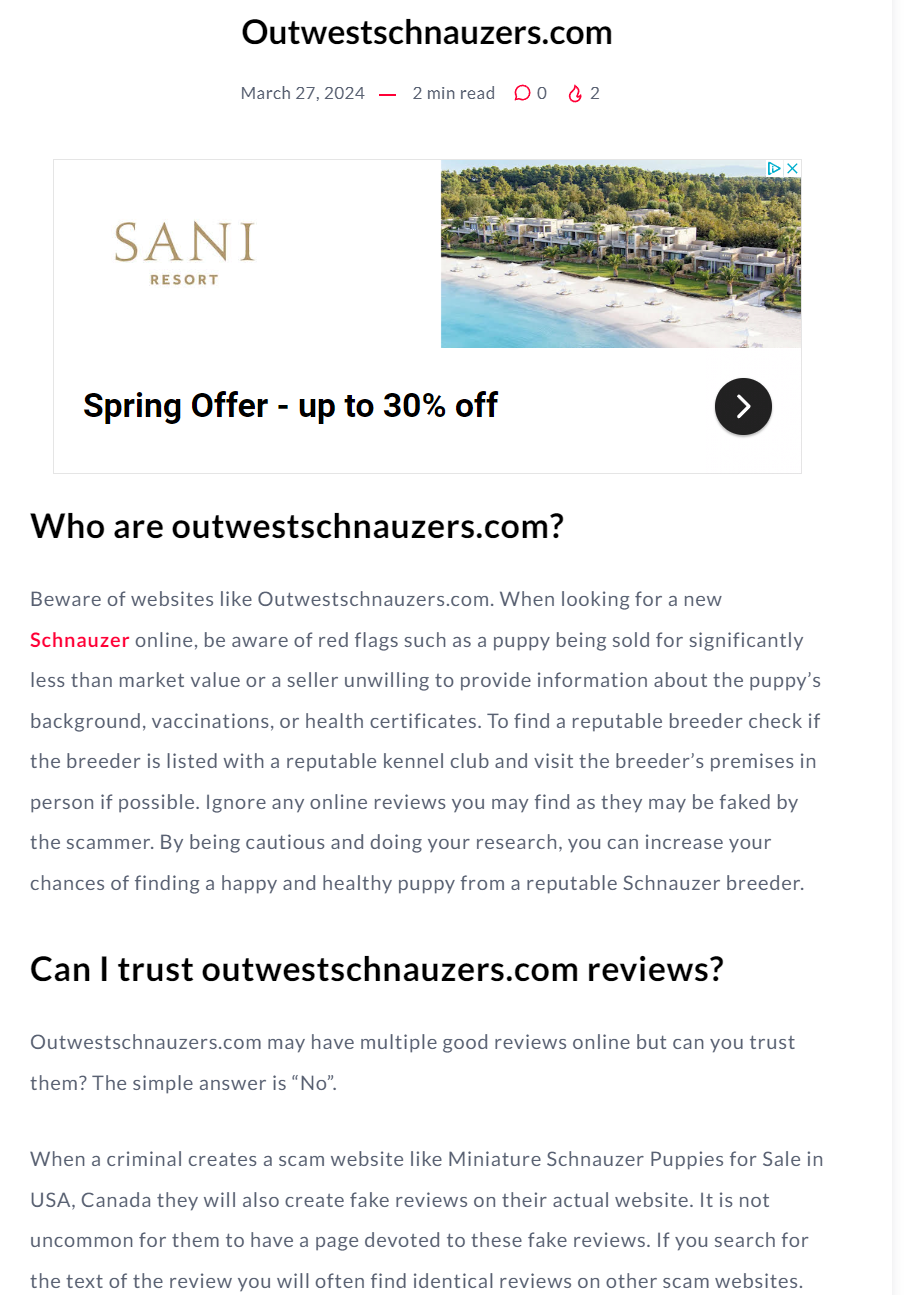
\includegraphics[width=\linewidth]{pic/figure3.png}
        \caption{Figure 3: Scam - Outwestschnauzers.com}
        \label{fig:sub3}
    \end{subfigure}
    \caption{Figure 2 (Homeafc.com) and Figure 3 (Homeafc.com)}
    \label{fig:main2}
\end{figure}

It is indicated that the function of ‘robots.txt’ is to tell search engines which URLs in the site are allowed for crawler access \cite{noauthor_robotstxt_nodate}. By visiting \url{https://petscams.com/robots.txt}, you can understand the scope of web crawling permissions set by the developers, and the text data returned in the page is as follows:
\vspace{10pt}

\noindent\hrule  
\begin{verbatim}
# START YOAST BLOCK
# ---------------------------
User-agent: *
Disallow:

Sitemap: https://petscams.com/sitemap_index.xml
# ---------------------------
# END YOAST BLOCK
\end{verbatim}
\hrule  
\vspace{10pt}


It can be seen that the configuration of the file is highly open. The rules specified by \url{www.petscams.com} permit all search engine crawlers to access all the content on the website, providing a solid foundation for the implementation of web scraping technologies.


\section{Web Scraping}
Compared to traditional manual data collection, web scraping can automatically retrieve unstructured data from a large amount of text such as HTML, then convert it into a structured format and store it locally \cite{khder_web_2021}. As Zhao stated \cite{zhao_web_2017}, the web scraping process mainly includes two parts: acquiring web resources and extracting specific information from the received data. The former refers to accessing the target webpage via the HTTP protocol, while the latter is to parse and extract the necessary data through automated scripts, and then save it in a specific format for further analysis. In this section, we will focus on discussing the most commonly used technology libraries when performing these two stages.
\\

In the first stage of web scraping, communication with the web server needs to be conducted through the HTTP, which is a request-response protocol that supports most web pages \cite{chandra_python_2015}. The Requests library in Python simplifies interaction with the target URL, providing efficient and reliable methods. As one of the most popular HTTP libraries, it supports the use of various HTTP methods, including GET, POST, PUT, and DELETE. Moreover, it also includes advanced features such as handling error and exception, authentication, redirects, sessions and SSL verification \cite{noauthor_requests_nodate}. These features meet all the requirements of the initial steps, ensuring the simplification of obtaining and processing server responses, including headers, session cookies, and status codes.
\\

For the second stage, various tech libraries can be utilised to parse and extract web data. Currently, BeautifulSoup, Selenium, and Scrapy are widely used because of their powerful capabilities. These tools focus on interactions with websites, as well as the extraction and parsing of data, each one demonstrating its own performance and advantages.
\\

BeautifulSoup is a Python library designed for parsing HTML and XML documents. It offers a simple and user-friendly syntax, enabling users to swiftly locate the necessary elements in the parsing tree using selectors like tag names, id names, etc \cite{chandra_python_2015}. For small or medium-sized crawling tasks on static web pages, BeautifulSoup can often be paired with the Requests library to form a lightweight crawling solution. It's important to note that this technology library primarily focuses on parsing work and does not involve constructing concurrent requests \cite{fariha_beautifulsoup_2023}.
\\

Similarly, Selenium does not support concurrent requests, which limits its efficiency in asynchronously executing multi-site scraping tasks to a certain extent. However, as a browser automation tool, Selenium supports multiple programming languages including Python, Java, and C\#, demonstrating unique capabilities in automating web browser operations \cite{fariha_beautifulsoup_2023}. Due to the unique support for JavaScript dynamically loaded pages \cite{fariha_beautifulsoup_2023}, it specialises in simulating human user actions, such as scrolling through pages, filling out forms, and clicking buttons. Additionally, unlike tools that need to be combined with the Requests library to send HTTP requests, scripts written by Selenium can run independently, using its built-in browser control functions to directly access and operate web pages. As the automated form filling will be introduced in project development, Selenium will become an indispensable tool library.
\\

Scrapy is a web crawler framework written in Python, which includes a complete set of web scraping solutions, including request handling mechanisms, data extraction, and database storage \cite{noauthor_intro_nodate}. Utilising the Twisted asynchronous network framework, Scrapy supports efficient concurrent request handling, making it particularly suitable for large-scale data crawling tasks and complex web data collection projects \cite{noauthor_intro_nodate}. Apart from being less self-sufficient in handling JavaScript than Selenium, and new users may encounter a certain learning curve, Scrapy better integrates the key functions of both Requests and BeautifulSoup. Thus, it can complete tasks independently in most scenarios without relying on external libraries.
\\

However, the demand of this project is relatively simple, there is no need to handle a large number of concurrent requests or complex data crawling. Therefore, I finally chose Requests, BeautifulSoup and Selenium as tools for the crawler development, since our main focus is to prioritise the smooth execution of the overall system process. While this approach may not be as comprehensive as Scrapy, it offers sufficient flexibility and convenience to meet project requirements. If necessary, it has also kept a door open for incorporating more efficient and complex crawling technologies in the future.


\section{Recognition and Processing of Text Data}
Throughout the construction and execution of the project system, various types of text data will be encountered, such as form content, email content, and time records. To manage these data effectively, this section introduces various methods for implementing information retrieval, guided by the heuristic search algorithm concept. These methods can be used separately or in combination, to ensure that the system identifies and processes text data accurately and efficiently.
\\

Heuristic search is a goal-oriented searching method. While it doesn't always guarantee the optimal solution, it usually provides high-quality solutions \cite{a_chapter_2001}. The heuristic search algorithm, also known as the A* algorithm, merges the benefits of keyword search and clustering. When dealing with NP problems that have incomplete solving conditions, the following evaluation function is established \cite{zhao_information_2014}:
\\

f(n)=g(n)+h(n)
\\

Here, f(n) represents the total estimated cost of node n, g(n) represents the actual path cost from the beginning state to node n, and h(n) stands for the heuristic estimated cost from node n to the goal. These values can help reflect the distance between the node and the goal, guiding the optimal path with each search step. This algorithm improves search efficiency by avoiding the exploration of invalid paths, thus improving the accuracy of vital information retrieval while ensuring the response speed. Therefore, the essence of heuristic search is to use limited information to achieve the search goal at the lowest cost. After acquiring substantial data through web scraping, this logic can also facilitate the fast batch retrieval of relevant information. Based on the characteristics or patterns of the data items, you can predefine the keyword groups, key data types, and different pattern matches. This allows scripts to execute "semi-structured" searches, effectively recognising and filtering vast amounts of text \cite{manning_introduction_2009}.
\\

Furthermore, the use of Regex and the FuzzyWuzzy library also demonstrates the application of heuristic search. As Uzum's report \cite{uzun_comparison_2018}, Regex is a sequence of characters that define a search pattern. With the introduction of the "re" module in Python, a pattern is predefined to extract data. However, this study also found that data extracted using Regex is only 43.5\% accurate compared to the expected data. Therefore, this project will consider using only simple Regex rules to remove unnecessary text information. 
\\

FuzzyWuzzy is a Python library used for string matching. Unlike Regex, once this library is utilised, a relevance score ranging from 0-100 need to be set \cite{majumder_fuzzywuzzy_2021}. The higher the score, the more closely the query word should match the target string. This can also be viewed as the retrieval constraints defined in retrieval heuristics \cite{yang_secure_2021}. By using fuzzy string matching, this heuristic method allows for a wider range of possibilities for a target string with uncertain content, thereby preventing over-matching a single query word.


\section{GPT Models}
In response to the demand for generating a large number of emails, the conventional approach involves using predefined text templates to generate email content. However, for a more advanced automated response system, I decided to integrate the GPT model.
\\

GPT, short for Generative Pre-Trained Transformer, has been extensively pre-trained on natural language data. It can predict and generate subsequent content after receiving text, images, or sound through the transformer \cite{3blue1brown_but_2024}. Since the release of the first GPT-1 version in June 2018, OpenAI has developed numerous models with various functions \cite{noauthor_openai_nodate}. For instance, the GPT series focuses on understanding and generating natural language or code; DALL·E specialises in image generation and editing; Whisper, a voice recognition model, and Jukebox is a music generation model. And these models are still being continuously updated and optimised.
\\

The core requirement of this project is to effectively understand and generate natural language text. In that case, the newly released GPT-3.5-turbo-0125 and GPT-4-0125-preview models both meet this requirement well. The processing capabilities of these two models have reached up to 60,000 tokens (approximately 45,000 English words) and 300,000 tokens (approximately 225,000 English words) per minute \cite{noauthor_openai_nodate}. This demonstrates that by integrating the API key into the system, adjusting both the necessary prompts and other parameters according to the code template provided by OpenAI \cite{noauthor_openai_nodate}, AI can automatically generate email content in batches using human language logic. Which will result in an efficient response speed and a natural interaction experience.




\chapter{Project Execution}
\section{Implementation of Web Scraping}
In this project, web scraping is primarily used to access, collect, and fill in a large amount of data on the form pages of pet scam websites. We have learned before that \url{www.petscams.com} is a key resource, dedicated to collecting and reporting information on scam websites related to pet sales and transportation. Given that pet transportation scams are often only involved in the later stages of scam activities, and these scam websites do not expect consumers to contact them proactively. Therefore, our crawlers will only focus on those fraudulent pet websites involved in sales.

\subsection{Crawling and Filtering List of Target Websites}
The initial step of the crawling process is handled by \texttt{petscam\_crawl.py}. The task of this script is to extract links from the target websites and store them in a JSON file for subsequent processing. As mentioned above, an HTTP request is first sent through the requests library to access the specific category page that lists fake pet sales websites, which is \url{https://petscams.com/category/puppy-scammer-list/}. Then the HTML source code obtained by the request is passed to a BeautifulSoup object and parsed with 'html.parser' as the parser. In analysing the structure of the \url{petscams.com} site, the program primarily locates the $<$article$>$ tag in the HTML. It then scans each $<$article$>$ tag for the $<$time$>$ tag, which contains the publication date, and also the $<$h2 class="main-title"$>$ tag that contains the website domain. This approach allows us to filter articles within a specific time frame based on their publication dates. Additionally, the \texttt{get\_text().strip()} method is incorporated into the code that only the domain name can be extracted from the text part in each $<$h2$>$ tag. This is followed by automatically prefixing 'https://' to each link to ensure direct accessibility.
\\

In the process of testing this script to scrape articles published within the past 30 days, a total of 460 scam domain names were successfully extracted. However, upon visiting some of these links randomly from our storage list, it was found that a number of them had already expired. This typically manifests as website access failure, return of 404 and other error status codes, or the website loading successfully but displaying messages such as "Account Suspended" or "Maintenance mode is on", suggesting that the domain name is temporarily unavailable. This issue is more prevalent in scam domain names that were revealed earlier. To enhance link crawling effectiveness, the code now includes checks for the return status code of the link and potential messages prompts. If the status code isn't 200 or the text returned by the request contains key messages provided, the relevant URL won't be saved. On the other hand, since the administrator of \url{www.petscams.com} occasionally re-post the same websites, which can lead to duplicate links in the processing list. The unique feature of a set is that it disallows duplicate elements \cite{sturtz_sets_nodate}. Hence, the solution is to initialise a set that stores all valid URLs. After that, convert this set to a list for storage in the target JSON file.
\\

After adjusting the code and confirming no new articles were being published, \texttt{petscam\_crawl.py} was run again. At this point, the program successfully removed 104 invalid links and 29 duplicates from the original 460, reducing the total number of links down to 327. These changes may have slightly impacted performance, increasing the crawler's running time. However, they effectively prevented the potential waste of time and decrease in accuracy that invalid or duplicate links could cause in the subsequent code execution process.


\section{Integrating Response Strategies}





\section{Construction and Operation of the System}





\chapter{Analysis of results}



\chapter{Critical Evaluation}









\chapter{Conclusion}





% \bibliographystyle{ieee}
\bibliography{references}

\appendix

\chapter{Appendix A: }
\label{}






\end{document}
